\documentclass[10pt,a4paper]{article}
\usepackage{ngerman}
\usepackage{sectsty, xcolor}
\usepackage{enumitem, fancyhdr, graphicx, lastpage}
\usepackage[hidelinks]{hyperref}
%\usepackage{authblk}

\definecolor{dunkelblau}{rgb}{0,0.4,0.6}
\subsectionfont{\color{dunkelblau}}

\title{ISF HS 2019}
\author{Victor Fernández\\Pavaskar Parameswaran}
\date{Dezember 2019}


\addtolength{\oddsidemargin}{-.875in}
\addtolength{\evensidemargin}{-.875in}
\addtolength{\textwidth}{1.75in}
\addtolength{\topmargin}{-.875in}
\addtolength{\textheight}{1.75in}

% muss nach Änderung der margin kommen!
\pagestyle{fancy}
\fancyhf{} %reset
\fancyhead[L]{HSLU}
\fancyhead[C]{ISF}
\fancyhead[R]{\thepage/\pageref{LastPage}}
\fancyfoot[L]{}
\fancyfoot[C]{}
\fancyfoot[R]{}
\renewcommand{\headrulewidth}{0.2pt} % Strich in Kopfzeile

%******
\begin{document}
\maketitle
\thispagestyle{empty}
\section*{Vorwort}Diese Zusammenfassung entstand in einer Gruppe während der Lernphase des HS 2019. Alle Fragen aus der Stoffabgrenzung tragen eine {\color{dunkelblau}blaue Farbe} und stehen als Unterkapitel. Das Dokument ist Open Source und jeder der möchte und signifikant beiträgt, darf sich als Autor anhängen. Die Source ist \underline{\href{https://github.com/vigi86/HSLU_Zusammenfassungen/tree/master/ISF_HS19}{dieses GitHub-Repo}}. Dies ist mein erstes \LaTeX{}-Dokument überhaupt. Nichts desto trotz wurde auf eine klare Strukturierung und Lesbarkeit des Dokumentes Wert gelegt.
\tableofcontents
\thispagestyle{empty}
\pagebreak

\part{Einführung (SW~01)}
\section{Einführung}
\subsection*{Einführung in das Thema "`Management von Informationssicherheit"'}
\paragraph*{Daten, Information und Wissen}
Information ist die Verknüpfung von Daten in Form von Zahlen, Worten und Fakten zu interpretierbaren Zusammenhängen.
Durch die Vernetzung von Informationen entsteht Wissen, das zunächst personenbezogen ist.
\paragraph*{Missbrauch}Informationen müssen vor Missbrauch geschützt werden
\begin{figure}[ht]
    \begin{center}
    \includegraphics[width=8cm]{images/Wissenspyramide.png}
    \caption{Wissenspyramide (Wikipedia)}
    \label{Wissenspyramide}
    \end{center}
\end{figure}


\subsection*{Motivation / Bedrohungen}
\paragraph*{Was gefährdet die Informationen?} Welche Gefährdungen/Bedrohungen gibt es?
\begin{itemize}[noitemsep,topsep=0pt,leftmargin=*]
    \item Nicht vorsätzliche (zufällige) Gefährdungen/Bedrohungen
    \begin{itemize}[noitemsep,topsep=0pt,leftmargin=*]
        \item Naturgewalten (Blitz, Hagel, Unwetter, Erdrutsche, Hochwasser, etc.)
        \item Ausfall von Strom oder Telekommunikation
        \item Technische Pannen, z.B. Fehler von Hard- und/oder Software
        \item Bedienerfehler / Fahrlässigkeit der Mitarbeitenden
    \end{itemize}
    \item Vorsätzliche Gefährdungen/Bedrohungen
    \begin{itemize}[noitemsep,topsep=0pt,leftmargin=*]
        \item Bösartiger Code (Viren, Würmer, Trojaner, etc.)
        \item Informationsdiebstahl
        \item Angriffe (von Skript-Kiddies bis Hacker)
        \item Wirtschaftsspionage ("`was die Konkurrenz wissen möchte"')
        \item Missbrauch der IT-Infrastruktur
    \end{itemize}
\end{itemize}

\subsection*{Grundbegriffe}
\textbf{Zutritts-, Zugangs-, Zugriffskontrolle}
\begin{itemize}[noitemsep,topsep=0pt,leftmargin=*]
    \item \textbf{\textsl{Zutrittskontrolle: }}Schutz des physischen Systems (Bsp. Serverraum)
    \item \textbf{\textsl{Zugangskontrolle: }}Schutz des logischen Systems (Bsp. Betriebssystem)
    \item \textbf{\textsl{Zugriffskontrolle: }}Daten-bezogen; Schutz der Operationen (Bsp. Dateisystem)
\end{itemize}


\part{Kryptographie (SW~02-04)}
\section{Symmetrische Kryptographie}
\subsection*{Sie verstehen was Steganographie ist}
\paragraph*{Steganographie}Verstecken von Information, z.B. in Bildern oder Audiofiles.
\subsection*{Sie verstehen was Private-Key-Kryptographie ist, welche Arten von Sicherheit es gibt und welche Angriffsarten auf Verschlüsselung existieren}
\paragraph*{Zeichencodierung}Kodierung (=Encoding) heisst, einen Wert mit Symbolen eines Zeichensatzes darzustellen. Beispiel:\\
\begin{tabular}{ |ll|}
    \hline
        Dezimalsystem & 100\\
        Binärsystem & 1100100\\
        Hexadezimalsystem (`hex') & 64\\
        ASCII & hello\\
        Base64 & aGVsbG8=\\
    \hline
\end{tabular}
{\color{red}\textbf{Achtung: Kodierung $\neq$ Verschlüsselung}}
\paragraph*{Symmetrische Verschlüsselung}Bei symmetrischen Verschlüsselungsverfahren gibt es im Gegensatz zu den asymmetrischen Verfahren, \textbf{nur einen einzigen Schlüssel}. Dieser Schlüssel ist für die Verschlüsselung, als auch für die Entschlüsselung zuständig.
\paragraph*{Secret Key Verschlüsselung}Secret Key (`Symmetrische') Verschlüsselung wird zwischen zwei Parteien verwendet, welche einen \textbf{gemeinsamen Schlüssel} besitzen. Ausserdem wird sie oft verwendet, wenn der gleiche Benutzer ein Dokument verschlüsseln und zu einem späteren Zeitpunkt wieder entschlüsseln muss.
\paragraph*{TODO}BILD\\


Private Key: Ein Kennwort, das benutzt wird, um einen Klartext zu verschlüsseln und so einen Geheimtext zu erhalten.
\paragraph*{TODO}BILDER


Jeder kann den öffentlichen Schlüssel zum Verschlüsseln verwenden. Nur der Besitzer des privaten Schlüssels kann entschlüsseln.

\subsection*{Sie können "`klassische"' symmetrische Verschlüsselungverfahren wie Ceasar cipher, Vigenère cipher, one-time pad anwenden und verstehen die Vor- und Nachteile bzw. Schwachstellen dieser Verfahren}
\paragraph*{Cesar cipher}Caesar-Verschlüsselung ist ein einfaches symmetrisches Verschlüsselungsverfahren, das auf der monographischen und monoalphabetischen Substitution basiert.\\
\textbf{Vorteil:} es ist \textbf{einfach}.\\
\textbf{Nachteil:} es ist \textbf{unsicher}, da es sehr schnell geknackt werden kann.\\
\textbf{Schwachstelle:} Die in der natürlichen Sprache ungleiche Verteilung der Buchstaben wird durch diese Art der Verschlüsselung nicht verborgen, so dass eine Häufigkeitsanalyse (Frequenzanalyse) das Wirken einer einfachen monoalphabetischen Substitution enthüllt.
\paragraph*{TODO}BILD: Schematische Darstellung einer Verschiebechiffre mit Verschiebung um 3 Buchstaben.\\

\noindent
Das folgende Diagramm zeigt die Häufigkeitsverteilung der Buchstaben in einem längeren Text in deutscher Sprache:
\paragraph*{TODO}BILD
\paragraph*{TODO}Wie zu erwarten, ist der häufigste Buchstabe E, gefolgt von N und I, wie es im Deutschen üblicherweise der Fall ist. Wird der Text mit dem Schlüssel 10 (oder anders gesagt, mit dem Schlüsselbuchstaben J) chiffriert, erhält man einen Geheimtext, der folgende Häufigkeitsverteilung besitzt: (BILD)


Der häufigste Buchstabe ist hier O, gefolgt von X und S. Man erkennt auf den ersten Blick die Verschiebung des deutschen "`Häufigkeitsgebirges"' um zehn Stellen nach hinten und besitzt damit den Schlüssel. Voraussetzung ist lediglich, dass man die Verteilung der Zeichen des Urtextes vorhersagen kann.


Besitzt man diese Information nicht oder möchte man auf die Häufigkeitsanalyse verzichten, kann man auch die Tatsache ausnutzen, dass bei der Cäsar-Chiffre nur eine sehr kleine Anzahl möglicher Schlüssel in Frage kommt. Da die Größe des Schlüsselraums nur 25 beträgt, was einer "`Schlüssellänge"' von nicht einmal 5~bit entspricht, liegt nach Ausprobieren spätestens nach dem 25. Versuch der Klartext vor.

\paragraph*{Cesar cipher: Vorgang}
\begin{itemize}[noitemsep,topsep=0pt,leftmargin=*]
    \item Verschiebt jeden Buchstaben des Alphabets um eine bestimmte Anzahl Stellen
    \item Soll bereits von Julius Caesar verwendet worden sein
    \item Der Schlüssel wird entweder als Anzahl Stellen, um die verschoben wird, oder als Buchstaben, auf den `A' verschoben wird angegeben
    \item Variante: ROT13 (Verschlüsselung = Entschlüsselung)
    \item Problem 1: Schlüssellänge (nur 26 verschiedene Schlüssel)
    \item Problem 2: Frequenzanalyse
\end{itemize}
\paragraph*{TODO}BILD aus Folie mit Cesar Verschiebung
\paragraph*{Vigenère cipher}
\begin{itemize}[noitemsep,topsep=0pt,leftmargin=*]
    \item Schlüssel: Wort der Länge $L$
    \item Jeder Buchstabe im Text wird mit der Cesar cipher des entsprechenden Schlüsselwortes verschlüsselt
    \item Anzahl mögliche Schlüssel: $26^L$
    \item Problem: Frequenzanalyse jeder $L$'ten Stelle
\end{itemize}
\paragraph*{TODO}BILD Vigenère cipher
\paragraph*{One-time pad}
\begin{itemize}[noitemsep,topsep=0pt,leftmargin=*]
    \item Jede Stelle wird mit einem anderen Schlüssel verschlüsselt
    \item Darf nur 1 Mal verwendet werden!
    \item Anzahl möglicher Schlüssel = Anzahl möglischer Nachrichten
    \item Ist sicher, d.h. Geheimtext verrät keinerlei (zusätzliche) Information über den Klartext
    \item Intuitiv: Für einen bestimmten Geheimtext sind \textbf{alle} Klartexte (dierser Länge) möglich
\end{itemize}
\paragraph*{TODO}BILD one-time pad

\subsection*{Sie wissen welche modernen Verschlüsselungsalgorithmen in der Praxis verwendet werden und was deren Eigenschaften sind}
\paragraph*{Informationstheoretische Sicherheit}Das Ziel informationstheoretischer Sicherheit ist der Schutz von Daten vor unbefugtem Zugriff während der Übertragung. Im Unterschied zur Kryptographie basiert informationstheoretische Sicherheit nicht auf der Annahme, dass die Rechenleistung eines unberechtigten Empfängers nicht gross genug ist, um die Daten zu decodieren. Vielmehr garantiert informationstheoretische Sicherheit, dass ein unberechtigter Empfänger selbst bei beliebig grosser Rechenleistung nicht in der Lage ist, solcherart geschützte Nachrichten zu decodieren. Mit anderen Worten erhält ein Angreifer durch den Geheimtext keinerlei (zusätzliche) Information über den Klartext. Beispielsweise ist OTP informationstheoretisch sicher.\newline
Formal:
\begin{math}
    P(M=m) = P(M=m|C=c)
\end{math} {\color{red}Erklärung der Variabeln??}
\paragraph*{Berechenmässige Sicherheit}Der sicheren Übertragung und Aufbewahrung vertraulicher Daten kommt in unserer von Information dominierten Gesellschaft immer grössere Bedeutung zu. Die heute gebräuchlichen Verfahren zur Datenverschlüsselung bieten allerdings nur beschränkte, sogenannt berechenmässige Sicherheit. Das bedeutet, dass diese prinzipiell von einem Angreifer, der über genügend Rechenleistung (zum Beispiel einen, heute noch hypothetischen, Quantencomputer) verfügt, gebrochen werden können.
\paragraph*{Kerckhoff's Prinzip}Der Angreifer kennt den Algorithmus und alle Details des Systems. Nur der Schlüssel ist geheim.
\paragraph*{Angriffsarten}Bei der Sicherheit von modernen Verschlüsselungssystemen wird zwischen den Angriffs-möglichkeiten des Angreifers unterschieden:
\begin{itemize}[noitemsep,topsep=0pt,leftmargin=*]
    \item \textbf{Ciphertext only attack:} Angreifer erhält nur den zu entschlüsselnden Geheimtext
    \item \textbf{Known plaintext attack:} Angreifer erhält zusätzlich andere Klartext-Geheimtext-Paare
    \item \textbf{Chosen plaintext attack:} Angreifer kann zusätzliche Klartexte wählen, zu denen er auch die Geheimtexte erhält
\end{itemize}
\paragraph*{TODO}ev. BILD zu Angriffsarten

\subsection*{Sie verstehen was eine Hashfunktion ist und welche Eigenschaften eine kryptographische Hashfunktion ausmachen, bzw. was es heisst, wenn eine Hashfunktion gebrochen ist}
\paragraph*{TODO}

\subsection*{Sie kennen moderne Hashfunktionen und wissen welche Eigenschaften diese haben}
\paragraph*{TODO}

\subsection*{Sie kennen Anwendungen von Hashfunktionen}
\paragraph*{TODO}

\subsection*{Sie wissen was ein keyed Hash (HMAC) ist und wofür dieser verwendet werden kann}
\paragraph*{TODO}

\subsection*{Sie kennen die "`Best-practices"' zu Passwortsicherheit und wissen, gegen welche Angriffe diese schützen}
\paragraph*{TODO}

\section{Asymmetrische Kryptographie}
\paragraph*{Asymmetische Verschlüsselung}In der asymmetrischen Kryptografie (Verschlüsselung) arbeitet man nicht mit einem einzigen Schlüssel, sondern mit einem \textbf{Schlüsselpaar}. Bestehend aus einem \textbf{öffentlichen} und einem \textbf{privaten Schlüssel}. Man bezeichnet diese Verfahren als asymmetrische Verfahren oder \mbox{Public-Key-Verfahren}.
\subsection*{Sie verstehen was Public-Key-Kryptographie ist, worauf deren Sicherheit basiert und wie sie zur Verschlüsselung, für Signaturen und zur Authentisierung verwendet werden kann}
\paragraph*{Public Key Verschlüsselung}Basiert auf Funktionen, welche einfach zu berechnen sind, deren Umkehrfunktion aber (vermutlich) schwierig zu berechnen ist.
Beispiel:\newline
\noindent
\begin{tabular}{|ll|}
    \hline
    Multiplikation (einfach):&$97\times84=8051$\\
    Faktorisieren (schwierig):&$8051=?$\\
    \hline
\end{tabular}
\paragraph*{TODO}BILDER aus "`The Science of Secrecy"'
\subsection*{Sie kennen die gängigen asymmetrischen Verschlüsselungs- und Signaturalgorithmen und wissen, worauf deren Sicherheit basiert}
\paragraph*{TODO}
\subsection*{Sie wissen wie Diffie-Hellmann-Schlüsselaustausch bzw. ElGamal-Verschlüsselung funktioniert}
\paragraph*{Diffie-Hellman (DH)}Diffie-Hellman ist ein Schlüsselvereinbarungsprotokoll. Der vereinbarte gemeinsame geheime Schlüssel kann danach zur Verschlüsselung der Nachricht verwendet werden.
\paragraph*{TODO}BILD \& ev. Beispiel Wiki
\paragraph*{ElGamal-Verschlüsselung}ElGamal verwendet DH um einen asymmetrischen Verschlüsselungsalgorithmus zu erstellen.
\paragraph*{TODO}BILD ElGamal
\paragraph*{TODO}ev. Beispielrechnung machen
\subsection*{Sie wissen was kryptographisch sichere Zufallszahlen sind und wo diese verwendet werden}
\paragraph*{TODO}
\subsection*{Sie wissen was eine elektronische Signatur ausmacht}
\paragraph*{TODO}
\subsection*{Sie wissen wie hybride Verschlüsselung bzw hybride Signaturen funktionieren}
\paragraph*{TODO}


\section{Zertifikate und SSL-TLS}
\subsection*{Sie kennen die verschiedenen Arten von "`Trust"'}
\paragraph*{TODO}
\subsection*{Sie wissen was eine Public-Key-Infrastruktur, eine Certificate Authority und ein Zertifikat ist, wofür und wie diese verwendet werden und wie Zertifikate ausgestellt und revoziert werden}
\paragraph*{TODO}
\subsection*{Sie wissen was SSL/TLS ist, welche Funktionalität es erreicht und wie das Protokoll konzeptionelle abläuft}
\paragraph*{TODO}



\part{Angriffe (SW~05-06)}
\section{Angriffe auf Webanwendungen}
\paragraph*{Bedrohungen auf Anwendungsebene}Webanwendung, Session, Headers, CSRF
\subsection*{Sie wissen was eine Webanwendung ausmacht, wie HTTP funktioniert}
Was unterscheidet eine Webanwendung aus Sicherheitssicht zu anderen Anwendungen?
\begin{itemize}[noitemsep,topsep=0pt,leftmargin=*]
    \item Kommuniziert über HTTP mit einem Server
    \begin{itemize}[noitemsep,topsep=0pt,leftmargin=*]
        \item zustandsloses Protokoll
    \end{itemize}
    \item Läuft in einem Browser
    \begin{itemize}[noitemsep,topsep=0pt,leftmargin=*]
        \item Mehrere Webanwendungen können parallel im gleichen Browser laufen
        \item Die Webanwendung \textsl{erbt} vom Browser implementierte Features
        bzw. muss diese richtig ansprechen
    \end{itemize}
\end{itemize}
\paragraph*{HTTP}Der Browser kommuniziert mit dem Webserver über das \textbf{Hypertext Transfer Protokoll (HTTP)}. HTTP besteht aus \textsl{Requests} und \textsl{Reponses}.
\paragraph*{HTTP-Request-Methoden}Die häufigsten HTTP-Request-Methoden sind \textbf{GET} und \textbf{POST}.
Es existieren aber auch \textbf{PUT, HEAD, DELETE, PATCH, OPTIONS}.
\paragraph*{GET}\texttt{https://www.hslu.ch/?p=5 HTTP/1.1\\User-Agent: Mozilla/5.0}
\begin{itemize}[noitemsep,topsep=0pt,leftmargin=*]
    \item Message Body: kein
    \item Ruft Daten vom Server ab
    \item Sollte Serverzustand nicht verändern
\end{itemize}
\paragraph*{POST}\texttt{https://www.hslu.ch/ HTTP/1.1\\
User-Agent: Mozilla/5.0}
\begin{itemize}[noitemsep,topsep=0pt,leftmargin=*]
    \item Message Body: \texttt{id=123\&pwd=password}
    \item Darf Serverzustand verändern
    \item Wird nicht gecachet
\end{itemize}
\paragraph*{Häufigste Reponse-Codes}
\begin{itemize}[noitemsep,topsep=0pt,leftmargin=*]
    \item 200 OK
    \item 204 No Content
    \item 301 Moved Permanently
    \item 302 Found (Vorher: "`Moved temporarely"')
    \item 304 Not Modified
    \item 400 Bad Request
    \item 403 Forbidden
    \item 404 Not Found
    \item 500 Internal Server Error
\end{itemize}
\paragraph*{HTTP Zustand} HTTP ist ein zustandsloses Protokoll, d.h. es hat kein `Gedächtnis', bzw. Erinnerung.
\begin{figure}[ht]
    \begin{center}
    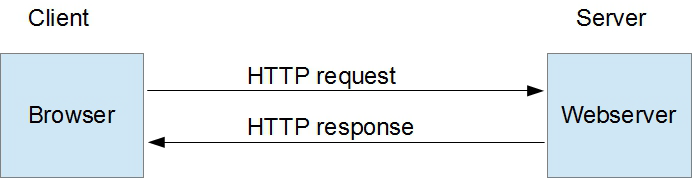
\includegraphics[width=12cm]{images/HTTPZustand0.png}
    \caption{HTTP zustandslos}
    \label{HTTPZustandslos}
    \end{center}
\end{figure}\\
Die einzige Möglichkeit einen Zustand an den Client zu übergeben ist, diesen per weiteren Requests mitzuschicken. Die Zustände werde mit einem Cookie oder einem "`Hidden field"' erfasst.
\begin{figure}[ht]
    \begin{center}
    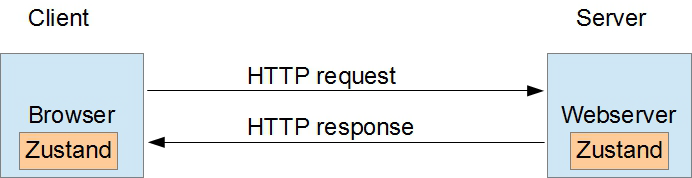
\includegraphics[width=12cm]{images/HTTPZustand1.png}
    \caption{HTTP Zustand per Request (hidden field)}
    \label{HTTPZustand}
    \end{center}
\end{figure}
\paragraph*{Cookies}Cookies sind kurze Textdaten, welche vom Server als Header an den Browser übermittelt werden und von diesem ebenso als Header bei requests wieder mitgesendet werden. Cookies werden vom Browser verwaltet. Die meistgenutzte Möglichkeit ist es, ein Cookie zu setzen. Jedoch dürfen auch Cookies nicht client-seitig angepasst werden können!
\begin{figure}[ht]
    \begin{center}
    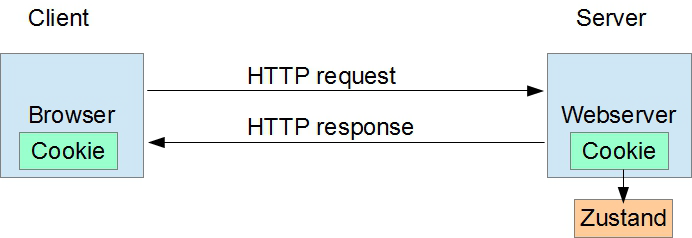
\includegraphics[width=12cm]{images/HTTPCookie.png}
    \caption{Einsatz eines Cookies}
    \label{HTTPCookie}
    \end{center}
\end{figure}
\paragraph*{Cookie Eigenschaften}Die Eigenschaften von Cookies sind:
\begin{itemize}[noitemsep,topsep=0pt,leftmargin=*]
    \item \textbf{Persistent} (mit Ablaufdatum) oder \textbf{Session-Cookie} (ohne Ablaufdatum)
    \item \textbf{Secure} (wird nur über HTTPS übertragen)
    \item \textbf{HTTP Only} (darf nur von HTTP gelesen werden)
    \item \textbf{Same Site} (wird nicht bei Cross-Domain-Aurfrufen mitgesendet, z.B. `embedded' Link, Image)
\end{itemize}

\subsection*{Sie wissen was eine Session ist und welche Eigenschaften einer Session bei welchen Angriffen wichtig sind bzw wie sie gegen gewisse Angriffe Schutz bieten}
\paragraph*{Session} Eine Session ist der Zeitraum, in dem ein Client eine stehende Verbindung mit einem Server hat; vom Login bis zum Logout. Der Server vergibt dem Client eine eindeutige Session-ID. Die Sitzungsdaten (z.B. Warenkorb) werden im Server gespeichert. Bei jedem Request gibt der Client seine Session-ID mit, damit der Server beim Response die zugehörigen Daten dieser ID übermitteln kann. Es gibt auch Sessions ohne stehende Verbindung (ohne Login). Dies wird zu Statistikzwecken verwendet, beispielsweise um die Bewegung des Besuchers auf der Website zu verfolgen. Oder aber auch um einen Warenkorb ohne Login verwenden zu können.
\paragraph*{Schwaches Session-Management}Was ist das?
\begin{itemize}[noitemsep,topsep=0pt,leftmargin=*]
    \item der Sessionwert ist vorhersagbar
    \item der Sessionwert kann vom Client gesetzt werden
    \item die Cookie-Attribute `Secure', `HttpOnly' oder `Same Site' sind nicht gesetzt
    \item Cookie-Domain oder -Pfad sind nicht so eingeschränkt wie möglich
    \item die Session wird bei einem Logout nicht invalidiert
    \item die Session hat kein server-seitiges Timeout (Inaktivitäts- und absolutes Timeout)
\end{itemize}
\paragraph*{Schwaches Session-Management}Was kann man dagegen tun?
\begin{itemize}[noitemsep,topsep=0pt,leftmargin=*]
    \item lange und kryptographisch zufällige Sessionwerte wählen
    \item nur vom Server gewählte Sessionwerte akzeptieren
    \item Cookies als `Secure',`HttpOnly' oder `Same Site' mit so eingeschränkter Domain und Pfad wie möglich setzten
    \item Session \textbf{server-seitig} bei einem Logout oder Timeout invalidieren
\end{itemize}
\paragraph*{Same Origin Policy}Mehrere Webanwendungen können im gleichen Browser parallel laufen. Die Same-Origin-Policy verhindert, dass eine parallel laufende Webanwendungen uneingeschränkt
\begin{itemize}[noitemsep,topsep=0pt,leftmargin=*]
    \item auf die Daten einer anderen Anwendung zugreifen
    \item die Cookies einer anderen Anwendung lesen oder mitschicken
    \item Requests auf die andere Anwendung absetzen
\end{itemize} kann.\\
Same Origin Policies im Browser gibt es z.B. für Cookies, DOM access (Zugang zu document.cookie), HTML5Storage, XMLHttpRequests.
\paragraph*{Same Origin Policy: Cookies} Cookies haben eine \textbf{domain} und \textbf{path}.
\begin{itemize}[noitemsep,topsep=0pt,leftmargin=*]
    \item \textbf{Setzen des Cookies:} Nur Domain-Suffix des URL-Hostname dürfen gesetzt werden. (Aber keine Top-Level Domains!)\\
    Path kann beliebig gesetzt werden.
    \item \textbf{Senden des Cookies:} Cookies werden dnur dann mitgeschickt, wenn die Cookie-Domain ein Domain-Suffix der URL-Domain und der Cookie-Path ein Prefix des URL-Path ist.
\end{itemize}
\paragraph*{Session Fixation}Was ist das?\\
Der Sessionwert wird nach einem Login oder Loginschritt nicht geändert. Ein  angreifer mit Zugang zu einer unauthentisierten Session kann warten bis ein Benutzer sich einloggt und ist damit selbst eingeloggt.
\paragraph*{Session Fixation}Was kann man dagegen tun?\\
Sessionwert nach jedem Authentisierungsschritt ändern.

\subsection*{Sie kennen sicherheitsrelevante Header}
\paragraph*{sicherheitsrelevante Response-Header}
\begin{enumerate}[noitemsep,topsep=0pt,leftmargin=*]
    \item \textbf{HSTS:} \texttt{Strict-Transport-Security:\\
    max-age=31536000; includeSubDomains}\\
    Seite wird nur via HTTPS aufgerufen. \texttt{max-age} muss hoch gesetzt werden!
    \item \textbf{Frame-Options:}\texttt{}
\end{enumerate}
\subsection*{Sie verstehen wie ein Cross-Site-Request-Forgery-Angriff abläuft und wie man sich dagegen schützen kann}
\paragraph*{TODO}


\section{Angriffe auf Protokollebene}
\subsection*{Sie kennen die Grundbegriffe der Anwendungssicherheit}
\paragraph*{TODO}
\subsection*{Sie kennen Beispiele von Angriffen auf verschiedenen Ebenen des Protokollstacks und wissen was diese bewirken}
\paragraph*{TODO}
\subsection*{Sie verstehen wie ein Cross-Site-Scripting / SQL-injection / Social-Engineering-Angriff abläuft und wie man sich dagegen schützen kann}
\paragraph*{TODO}



\part{Management (SW~07-09)}
\section{Standards \& Frameworks, ISMS}
\subsection*{Sie wissen, was ein ISMS ist und wie man damit umgeht}
\paragraph*{TODO}
\subsection*{Sie kennen die wichtigsten Standards der Informationssicherheit}
\paragraph*{TODO}
\subsection*{Sie finden sich in den Standards ISO 27001 und 27002 zurecht}
\paragraph*{TODO}
\subsection*{Sie verstehen die Grundzüge der BSI-Standards (BSI=Bundesamt für Sicherheit in der Informationstechnik, Deutschland)}
\paragraph*{TODO}
\subsection*{Sie kennen die Struktur und Grundziele des NIST CyberSecurityFrameworks}
\paragraph*{TODO}


\section{Risiko-Management und IT-Grundschutz}
\subsection*{Das Risikoanalyse-Verfahren verstehen}
\paragraph*{TODO}
\subsection*{Die Unterschiede zum Grundschutzverfahren kennen}
\paragraph*{TODO}
\subsection*{Eine einfache Risikoanalyse durchführen können}
\paragraph*{TODO}
\subsection*{Sie verstehen die Idee, die Ziele und die Konzepte des IT-Grundschutz-Vorgehens}
\paragraph*{TODO}
\subsection*{Sie kennen den Aufbau der IT-Grundschutz-Kataloge und deren Anwendungsweise}
\paragraph*{TODO}
\subsection*{Sie können die Teilschritte zum Aufbau eines Sicherheitskonzeptes nach IT-Grundschutz durchführen, kombinierte Risikoanalyse}
\paragraph*{TODO}


\section{Awarness}
\subsection*{Sie verstehen die Wichtigkeit der \flqq Awareness \frqq}
\paragraph*{TODO}
\subsection*{Sie kennen verschiedene Prozesse und Vorgehensweisen für die Initiierung, Durchführung und Erfolgsprüfung einer Awareness-Kampagne und können diese anwenden}
\paragraph*{TODO}
\subsection*{Sie kennen die relevanten Erfolgsfaktorender Mitarbeiter-Sensibilisierung und -Schulung und können diese in einer Kampagne umsetzen}
\paragraph*{TODO}



\part{Access Control (SW~10)}
\section{Access Control}
\subsection*{Sie kennen verschiedene Arten der Authentisierung, wissen wie diese technisch ablaufen und was deren Vor- und Nachteile sind}
\paragraph*{TODO}
\subsection*{Sie wissen wie verschiedene Authentisierungstoken technisch funktionieren, was deren Vor- und Nachteile sind und wie sie beim Login oder bei der Transaktionsbestätigung im e-Banking eingesetzt werden}
\paragraph*{TODO}
\subsection*{Sie wissen was Authentisierung, Autorisierung ist, warum diese wichtig sind und wie Angriffe darauf ablaufen}
\paragraph*{TODO}


\part{Multi-Party-Computation (SW~11)}
\section{Cryptographic Protocols}
\subsection*{Sie kennen einfache Beispiele von verteilten sicheren Berechnungen und verstehen wie die entsprechenden Protokolle ablaufen}
\paragraph*{TODO}
\section{Secret Sharing}
\subsection*{Sie kennen Arten von Sicherheit von verteilten sicheren Berechnungen und wie diese angegriffen werden können}
\paragraph*{TODO}
\subsection*{Sie wissen welche Eigenschaften elektronisches Geld ausmachen und kennen die technischen Grundlagen von Bitcoin}
\paragraph*{TODO}
\section{Zero Knowledge Proof}
\subsection*{Sie wissen was Zero-Knowledge-Proofs sind und wie diese ablaufen}
\paragraph*{TODO}



\part{Quantum (SW~12)}
\section{Quantum Computing and Quantum Cryptography}
\subsection*{Sie wissen was ein Quantencomputer ist und was ihn von einem "`klassischen"' Computer unterscheidet}
\paragraph*{TODO}
\subsection*{Sie verstehen welchen Einfluss die Existenz eines Quantencomputers auf die Kryptographie hat}
\paragraph*{TODO}
\subsection*{Sie verstehen wie Quantenschlüsselaustausch funktionert}
\paragraph*{TODO}
\part{WAF, Federations (SW~13)}
\section{Firewalls}
\subsection*{Sie wissen was die Aufgaben einer Firewall sind}
\paragraph*{TODO}
\subsection*{Sie verstehen die Funktionsweise einer WAF und wie sie eine Webanwendung vor Angriffen schützen kann}
\paragraph*{TODO}


\section{Federations}
\subsection*{Sie verstehen wie Authentisierung mit Identity Federation abläuft, was die Voraussetzungen dafür sind und was die Vor- und Nachteile von Federations sind}
\paragraph*{TODO}



\part{Talks (SW~14)}
\section{Malware}
\subsection*{Sie verstehen, welche Arten von Malware es gibt, welche Massnahmen gegen Malware sinnvoll sind und wie diese wirken}
\paragraph*{TODO}

\section{WAF}
\subsection*{Sie verstehen wo Machine-Learning in einer WAF eingesetzt werden kann und was einene Machine-Learning-Ansatz vom "`herkömmlichen"' Einsatz einer WAF unterscheidet}
\paragraph*{TODO}
\subsection*{Sie kennen Beispiele von Angriffen, welche mittels Machine-Learning auf einer WAF erkannt werden konnten}
\paragraph*{TODO}
\end{document}